\documentclass{beamer}

\title[ML and OT for shape parametrization]{Machine Learning and Optimal Transport for shape parametrization}
\author[G. Padula]{\textbf{Guglielmo Padula}\inst{1} \and Francesco Romor\inst{2}\and Giovanni Stabile\inst{2} \and Gianluigi Rozza\inst{2}}
\institute{\inst{1} University of Trieste, Italy (Intership at SISSA mathLab) \and \inst{2} Mathematics Area, mathLab, SISSA, International School of Advanced Studies, Trieste, Italy }

\date{}
\usetheme{Copenhagen}
\usepackage{graphicx}
\usepackage{tikz}
\usepackage{animate}
\usetikzlibrary{positioning,arrows.meta,quotes}
\usetikzlibrary{shapes,snakes}
\usetikzlibrary{bayesnet}
\tikzset{>=latex}
\tikzstyle{plate caption} = [caption, node distance=0, inner sep=0pt,
below left=5pt and 0pt of #1.south]
\begin{document}
\begin{frame}
\titlepage
\begin{center}

\includegraphics[height=4em]{logo_PyGeM.png}

\includegraphics[height=4em]{logo-mathlab_no_borders}

\includegraphics[height=4em]{logo_uni}

\includegraphics[height=4em]{logo_sissa_cerchio}
\end{center}
\end{frame}
\begin{frame}{Line 1: Semi-discrete Optimal Transport}
\textbf{Optimal transport map} definition:
$$\inf \left\{\int_{X} c(x, T(x)) \mathrm{d} \mu(x) \mid T_{*}(\mu)=\nu\right\}$$\\$\null$\\
\begin{itemize}
\item Regularity constraints
\item Application to design optimization
\end{itemize}$\null$\\
\centering
\animategraphics[loop,width=4cm]{100}{}{1}{100}

\end{frame}

\begin{frame}{Line 2: Generative models}
\textbf{Generative models} for shape optimization of complex geometries with a large number of parameters.
\begin{itemize}
\item Variational autoencoders:\\$\null$\\
\begin{tikzpicture}[thick,scale=0.5, every node/.style={scale=0.5},
squarednode1/.style={trapezium,draw=blue!60, fill=blue!60, very thick, minimum size=5mm},
squarednode2/.style={trapezium,draw=yellow!60, fill=yellow!60, very thick, minimum size=5mm},
]
\node[inner sep=0pt] (p11) {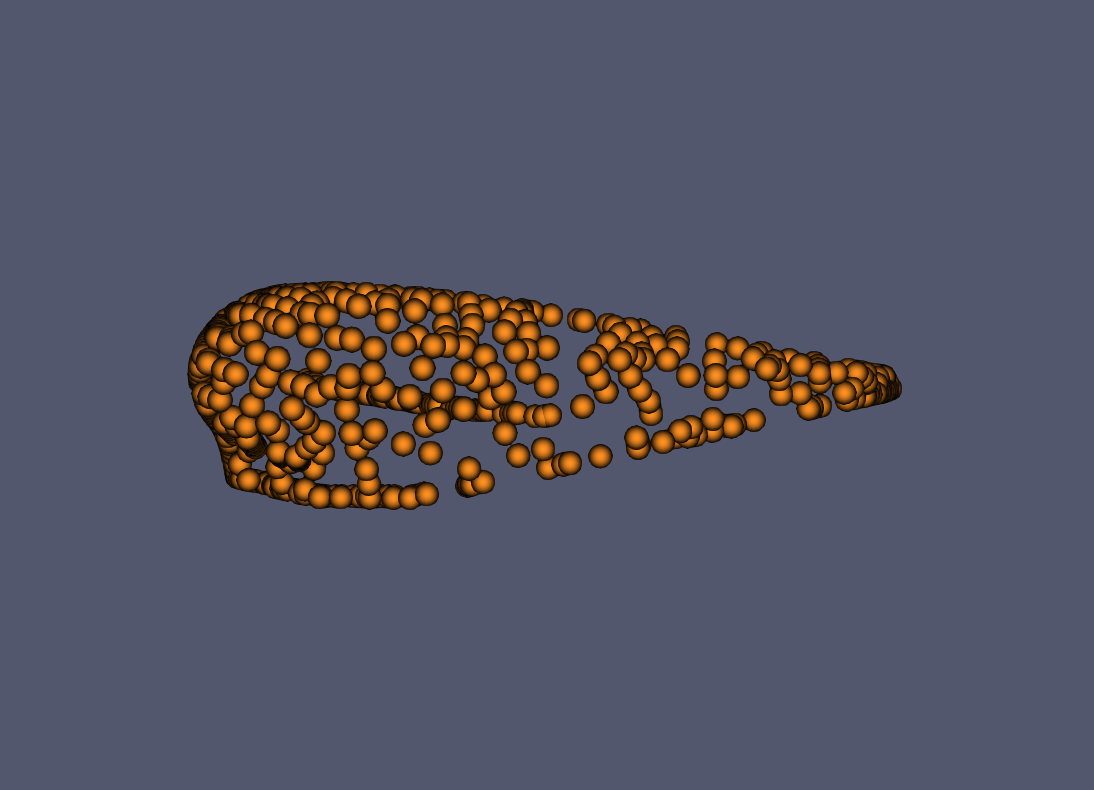
\includegraphics[scale=0.10]{mesh0}};
\node[squarednode1, rotate=90,left=of p11,shift={(-1,0)}]      (encoder)       [right=of p11]{\textbf{Encoder	}};
\node[inner sep=0pt,shift={(0,-1)}] (normal)  [right=of encoder]{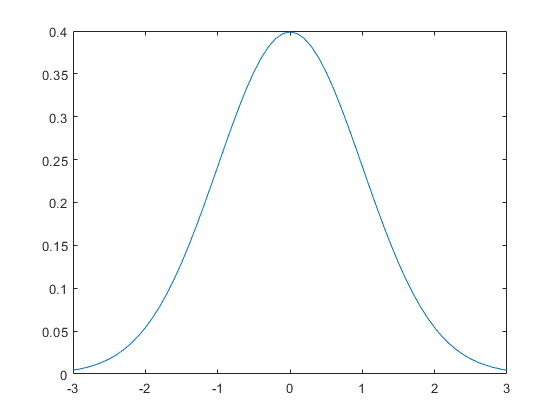
\includegraphics[scale=0.15]{normal}};
\node[squarednode2,rotate=-90,shift={(-1,0)}]      (decoder)       [right=of normal]{\textbf{Decoder}};
\node[inner sep=0pt,shift={(0,+1)}] (p21) [right=of decoder]{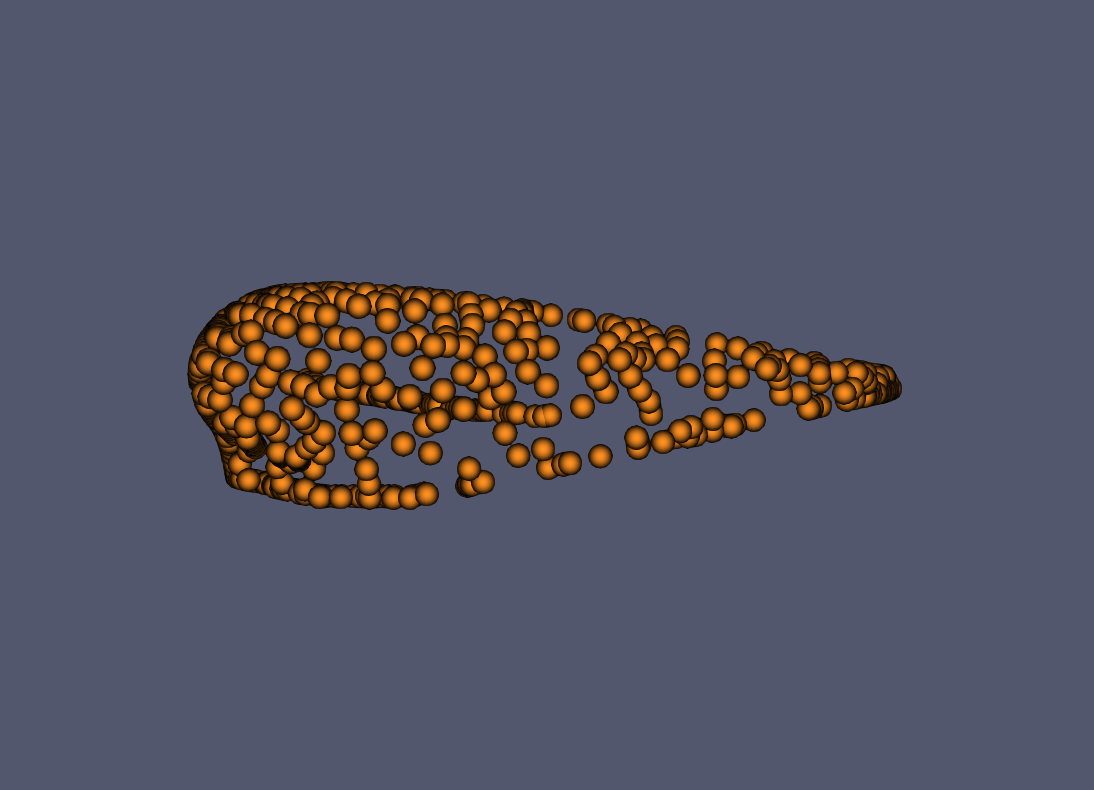
\includegraphics[scale=0.10]{mesh0}};

\draw[->] (p11.east) -- (encoder.north);
\draw[->] (encoder.south)-- (normal.west);
\draw[->] (normal.east) -- (decoder.south);
\draw[->] (decoder.north) -- (p21.west);
\end{tikzpicture}

\item Generative adversarial networks:\\$\null$\\
\begin{tikzpicture}[thick,scale=0.5, every node/.style={scale=0.5},
bluesquarednode/.style={rectangle, draw=orange!60, fill=orange!60, very thick, minimum size=5mm},
redsquarednode/.style={circle, draw=red!60, fill=red!60, very thick, minimum size=5mm},]


\node[inner sep=0pt] (normal) {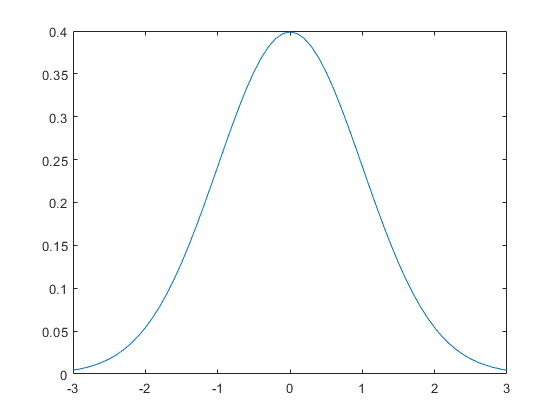
\includegraphics[scale=0.15]{normal}};
\node[bluesquarednode,rotate=-90,shift={(-1,0)}]      (generator)       [right=of normal]{\textbf{Generator}};
\node[inner sep=0pt,shift={(0,+1	)}] (mesh)  [right=of generator]{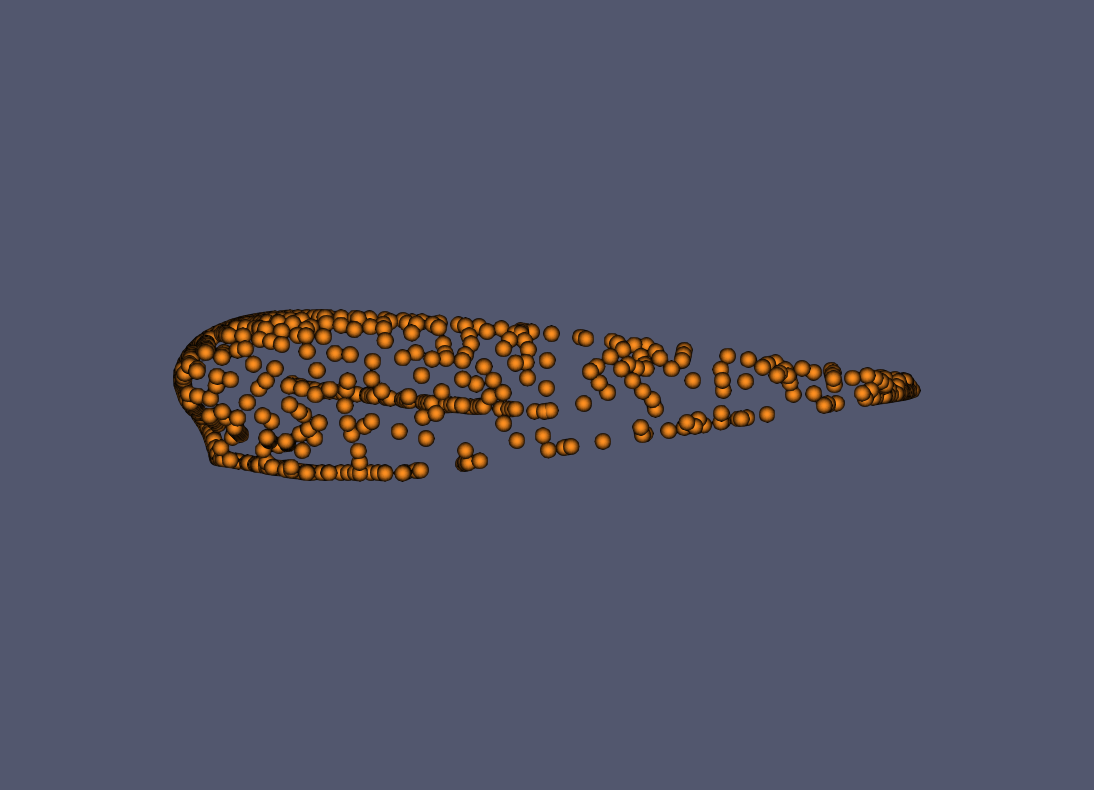
\includegraphics[scale=0.10]{mesh1}};
\node[bluesquarednode,rotate=-90,shift={(-1.32,0)}]      (discriminator)       [right=of mesh]{\textbf{Discriminator}};
\node[redsquarednode,shift={(0,1.32)}]      (false)       [right=of discriminator]{FALSE};

\draw[->] (normal.east) -- (generator.south);
\draw[->] (generator.north) -- (mesh.west);
\draw[->] (mesh.east) -- (discriminator.south);
\draw[->] (discriminator.north) -- (false.west);
\end{tikzpicture}\\$\null$ \\\begin{tikzpicture}[thick,scale=0.5, every node/.style={scale=0.5},
bluesquarednode/.style={rectangle, draw=orange!60, fill=orange!60, very thick, minimum size=5mm},
greensquarednode/.style={circle, draw=green!60, fill=green!60, very thick, minimum size=5mm},]


\node[inner sep=0pt] (cad)  {
\includegraphics[scale=0.10]{cad}};
\node[inner sep=0pt] (mesh)  [right=of cad]{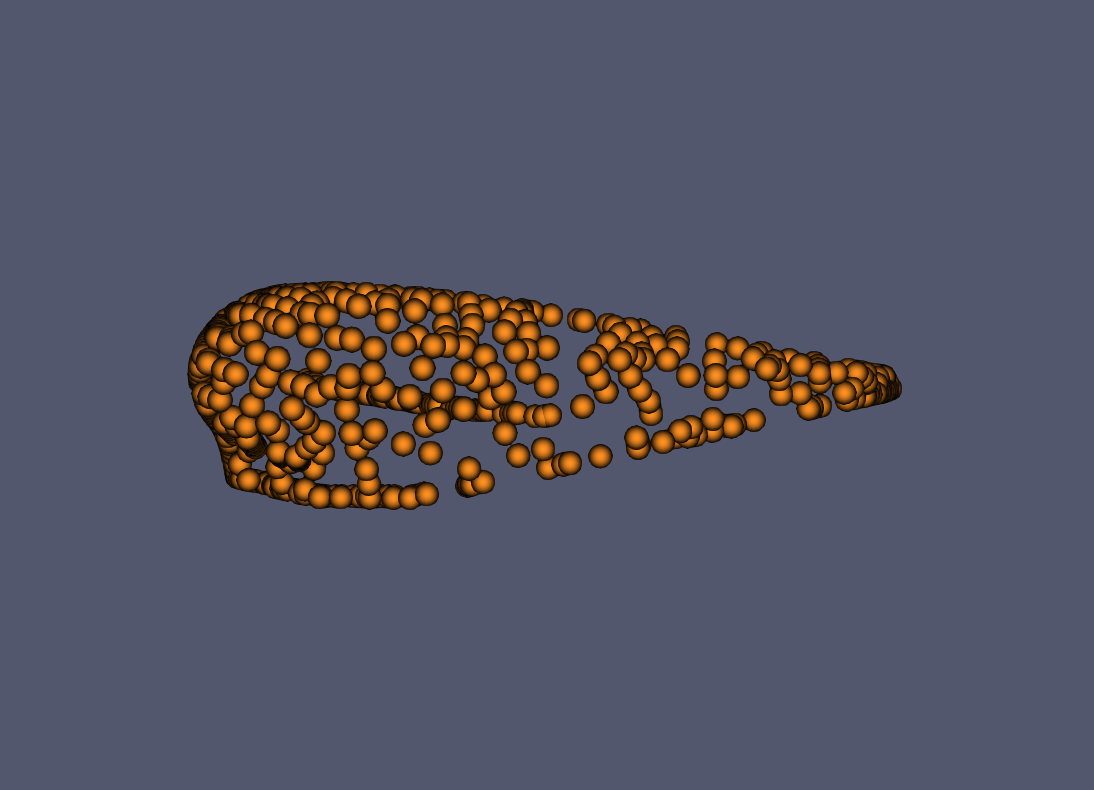
\includegraphics[scale=0.10]{mesh0}};
\node[bluesquarednode,rotate=-90,shift={(-1.32,0)}]      (discriminator)       [right=of mesh]{\textbf{Discriminator}};
\node[greensquarednode,shift={(0,1.32)}]      (false)       [right=of discriminator]{TRUE};

\draw[->] (cad.east) -- (mesh.west);
\draw[->] (mesh.east) -- (discriminator.south);
\draw[->] (discriminator.north) -- (false.west);
\end{tikzpicture} 
\end{itemize}
\end{frame}
\end{document}